\documentclass[svgnames,14pt]{beamer}

\usepackage{natbib}
\usepackage{amssymb}
\usepackage{amsmath}
\usepackage{amsthm}
\usepackage{graphicx}
\usepackage{setspace}
\usepackage{array}
\usepackage{tabularx}
\usepackage{verbatim}


\newcommand\dnr{\ensuremath{\mathit{DNR}}}
\newcommand\fail{\mathit{FAIL}}
\newcommand\pass{\mathit{PASS}}
\newcommand\defined{\mathrel{\;\stackrel{\scriptscriptstyle\mathbf{def}}{=}\;}}

\newtheorem{thm}{Theorem}
\theoremstyle{definition}
\newtheorem{defn}{Definition}

\mode<presentation>
{
  %%\usetheme{Madrid}
  \usetheme{Boadilla}
  %%\usetheme{Malmoe}
  %%\usetheme{Copenhagen}
  \setbeamercovered{dynamic}
  \setbeamertemplate{itemize items}[default]
  \usefonttheme{structurebold}
  \fontsize{10}{5}\selectfont
}

\title{Finding the Signal}
\subtitle{Improved Ranking and Noise Reduction in Black Box Testing}
\author{Jesse Welch}
\date{May 2012}

\advance\extrarowheight by 1.5pt

\begin{document}

\begin{frame}
\maketitle
\end{frame}


\begin{frame}
\frametitle{Students turn in many solutions \\ to the same problem}
We \only<1>{want to:}\only<2->{\textbf{really} want to}
\begin{itemize}
\item Test them \only<2->{\textbf{cheaply}}
\item Rank them \only<2->{\textbf{cheaply}}
\item Diagnose their faults \only<2->{\textbf{cheaply}}
\end{itemize}
\end{frame}

\begin{frame}
\begin{itemize}
\frametitle{Overview}
\item \only<1>{Intro to Ranking}\only<2>{Intro to Ranking}
\item \uncover<1>{Ranking with Multiple Results}
\item \uncover<1>{Union* Reduction}
\item \uncover<1>{Witness Reduction}
\end{itemize}
\end{frame}

\begin{frame}
\frametitle{There are many ways to rank}
\begin{itemize}
\item \uncover<2->{Number of tests passed}
\uncover<3->{\item Expert opinion}
\uncover<4->{\item Desperate, custom measures}
\end{itemize}
\end{frame}

\begin{frame}
\frametitle{There is a central truth}
In every one of these ranking algorithms,
$$\pass>\fail$$
\end{frame}

\begin{frame}
\frametitle{There is a central truth}
\begin{block}{}
$$S_1 \sqsubseteq S_2 \defined \forall t \in T : S_1(t) \leq S_2(t)$$
\end{block}
\end{frame}

\begin{frame}
\centerline{\includegraphics[height=\textheight]{rank1.ps}}
\end{frame}

\begin{frame}
\begin{itemize}
\frametitle{Overview}
\item \uncover<0>{Intro to Ranking}
\item Ranking with Multiple Results
\item \uncover<0>{Union* Reduction}
\item \uncover<0>{Witness Reduction}
\end{itemize}
\end{frame}


\begin{frame}
\frametitle{Real tests have many outcomes}
\begin{itemize}
\item Pass
\item \uncover<2->{Bad output}
\item \uncover<3->{Segfault}
\item \uncover<4->{Timeout}
\item \uncover<5->{Assertion failure}
\end{itemize}
\end{frame}

\begin{frame}
\frametitle{We pick an order}
Always:
\begin{itemize}
\item $\pass>\fail$
\end{itemize}
Sometimes:
\begin{itemize}
\item SEGFAULT $>$ BAD OUTPUT
\item BAD OUTPUT $>$ SEGFAULT
\end{itemize}
\end{frame}

\begin{frame}
\frametitle{How does this change ranking?}

\begin{center} 
\begin{tabular}{cc}
\includegraphics[width=0.35\textwidth]{rank1.ps}
&
\includegraphics[width=0.35\textwidth]{rank2.ps}\\
Single &
Multiple \\
\end{tabular}
\end{center}

\end{frame}

%TODO: Good example

\begin{frame}
\begin{itemize}
\frametitle{Overview}
\item \uncover<0>{Intro to Ranking}
\item \uncover<0>{Ranking with Multiple Results}
\item Union* Reduction
\item \uncover<0>{Witness Reduction}
\end{itemize}
\end{frame}

\begin{frame}
\centerline{\includegraphics[height=0.9\textheight]{fail.ps}}
\end{frame}

\begin{frame}
\frametitle{Some test sets are extremely large}
\begin{tabular}{ | l | c | }
\hline
Dataset & \#~Tests \\ 
\hline
bitpack & 2468 \\
divtest & 2112 \\
\hline
\end{tabular}
\end{frame}

\begin{frame}
\frametitle{Many tests are equivalent}
\begin{block}{}
$$ T_0 \equiv T_1 \defined \forall s \in S : s(T_0) \equiv s(T_1) $$
\end{block}
\end{frame}

\begin{frame}
\def\?{\phantom0}
\begin{tabular}{ | l | c | c | }
\hline
Dataset & \#~Tests & \#\ Classes\\ 
\hline
bitpack & 2468 & 144 \\
divtest & 2112 & \?71\\
\hline
\end{tabular}
\end{frame}

\begin{frame}
\frametitle{Some tests aggregate information}
If a program has two bugs (A,B), how can tests interact with them?
\begin{itemize}
\item \uncover<2->{Test neither bug}
\item \uncover<3->{Test bug A}
\item \uncover<4->{Test bug B}
\item \uncover<5->{Test both bugs}
\end{itemize}
\end{frame}

\begin{frame}
\frametitle{Why test both bugs?}
\begin{block}{}
A test $T_0$ is redundant if
\newline
$\fail (T_0) \equiv \fail(T_1) \cup \fail(T_2)$
\end{block}
\end{frame}

\begin{frame}
\def\?{\phantom0}
\begin{tabular}{ | l | c | c | c | }
\hline
Dataset & \#~Tests & \#\ Classes & Claessen\\ 
\hline
bitpack & 2468 & 144 & 91\\
divtest & 2112 & \?71 & 40\\
\hline
\end{tabular}
\end{frame}

\begin{frame}
\frametitle{Union*}
Why limit to only two aggregated tests?
\uncover<2->{
\begin{block}{}
A test $T_0$ is redundant if
\newline
$\fail (T_0) \equiv \fail(T_1) \cup \fail(T_2) \cup ... \cup \fail(T_n) $
\end{block}
}
\end{frame}

\begin{frame}
\def\?{\phantom0}
\begin{tabular}{ | l | c | c | c | c |}
\hline
Dataset & \#~Tests & \#\ Classes & Claessen & Union*\\ 
\hline
bitpack & 2468 & 144 & 91 & 87\\
divtest & 2112 & \?71 & 40 & 40\\
\hline
\end{tabular}
\end{frame}

\begin{frame}
\frametitle{Union* is \emph{never} worse}
Because it is a generalization of Claessen, Union* can never create a larger test set.
\end{frame}

\begin{frame}
\frametitle{Experimental effects}
\begin{itemize}
\item \uncover<2->{21 datasets}
\item \uncover<3->{18 reduced the same}
\item \uncover<3->{3 Union* reduced further}
\item \uncover<4->{Average of 3 additional tests reduced}
\end{itemize}
\end{frame}

\begin{frame}
\centerline{\includegraphics[height=\textheight]{success.ps}}
\end{frame}

\begin{frame}
\begin{itemize}
\frametitle{Overview}
\item \uncover<0>{Intro to Ranking}
\item \uncover<0>{Ranking with Multiple Results}
\item \uncover<0>{Union* Reduction}
\item Witness Reduction
\end{itemize}
\end{frame}

\begin{frame}
\frametitle{We want diagnostic information}
Ideally, this information is a list of bugs.
\newline\newline
Realistically, this information is a list of failed tests.
\end{frame}

\begin{frame}
\frametitle{This list can be extremely long}
A naive implementation would give the test result for every test failed.
\newline\newline
A reduced implementation gives a result only for each class of test that is used for the ranking graph.
\end{frame}


\begin{frame}
\def\?{\phantom0}
\centering
\begin{tabular}{ | l | r | r |}
\hline
Test & Failed Tests & Failed Classes \\
\hline
bitpack & 175.28 & 15.2 \\
divtest & 164.34 & 10.77 \\
\hline
\end{tabular}
\end{frame}

\begin{frame}
\frametitle{But can we do better?}
Tests are sometimes redundant for \emph{some} students.
\end{frame}

\begin{frame}
\frametitle{$\eta$-reduction}
$$T_1 : \lambda a.M_\eta a \longrightarrow M_\eta$$
$$T_2 : \lambda x.\lambda x.\lambda a.M_\eta a \longrightarrow \lambda x.\lambda x.M_\eta$$
\end{frame}

\begin{frame}
\verbatiminput{unreduced.witness}
\end{frame}

\begin{frame}
\frametitle{One outcome can \emph{imply} another}
\begin{block}{}
$$O_1 \Rightarrow O_2 \defined \forall s \in S : s(T_1) = O_1 : s(T_2) = O_2$$
\end{block}
\end{frame}

\begin{frame}
\frametitle{We can include only the implying failure}
\begin{block}{}
$$\forall T_1, T_2 \in W' : T_1 \not\Rightarrow T_2$$
\end{block}
\end{frame}

\begin{frame}
\verbatiminput{reduced.witness}
\end{frame}

\begin{frame}
\def\?{\phantom0}
\centering
\begin{tabular}{ | l | r | r | r |}
\hline
Test & Failed & Failed  & Reduced \\
     & Tests  & Classes & Witnesses \\
\hline
bitpack & 175.28 & 15.2 & 2.64\\
divtest & 164.34 & 10.77 & 1.65\\
\hline
\end{tabular}
\end{frame}

\begin{frame}
\frametitle{Experiment}
One one dataset, how well do these reductions correspond to expert knowledge?
\end{frame}

\begin{frame}
\frametitle{Results}
\begin{itemize}
\item 447 reductions
\item \uncover<2->{264 confirmed by expert}
\item \uncover<3->{59.1\% accuracy}
\end{itemize}
\end{frame}

\begin{frame}
\frametitle{\only<1>{There are 4 kinds of implications}\only<2>{We want 1 kind of implication}}
\begin{itemize}
\item \uncover<1>{Trivial}
\item \uncover<1>{Bogus}
\item \uncover<1>{Accidental}
\item \uncover<1->{Real}
\end{itemize}
\end{frame}

\begin{frame}
\frametitle{Important heuristic}
We remove every implication that comes from "know one thing about Matt, know everything about Matt".
\end{frame}

\begin{frame}
\frametitle{Results}
\begin{itemize}
\item 422 reductions
\item \uncover<2->{264 confirmed by expert} \only<3->{(the same number)}
\item \uncover<4->{62.5\% accuracy}
\end{itemize}
\end{frame}

\begin{frame}
\frametitle{We can improve the implications further}
The more negative implications we can find heuristics for, the better our accuracy will get!
\end{frame}

\begin{frame}
\frametitle{Conclusions}
\begin{itemize}
\item We can find more information than $\pass/\fail$
\item We can algorithmically produce and simplify a ranking of solutions \only<2->{\textbf{cheaply}}
\item We can algorithmically produce and simplify a diagnostic set of failures for each solution \only<2->{\textbf{cheaply}}
\end{itemize}
\end{frame}

\end{document}
